\documentclass[a4paper,twoside,12pt,fleqn]{scrartcl}
\usepackage[margin=2.5cm]{geometry}
%\usepackage{fancyref}
%\usepackage{graphicx}
%\usepackage{float}
%\usepackage{tabularx}
%\usepackage{booktabs,array}
%\usepackage{caption}
\usepackage{subcaption}
\usepackage{amsmath}
\usepackage{amsthm}
\usepackage{amssymb}
\usepackage{mathtools} % for multlined enviornment
%\usepackage{amsfonts}
%\usepackage{enumitem}
\usepackage[hyphens]{url}
\geometry{a4paper}
\usepackage{amssymb}%---allows \mathbb{R/Z/etc.} (numbers sets)
\usepackage{scrextend} %for eddmargin environment
\usepackage{caption}
\usepackage{titlesec}


%%%%[for python code] %%%%%%
\usepackage{listings}
\usepackage{color}

\definecolor{dkgreen}{rgb}{0,0.6,0}
\definecolor{gray}{rgb}{0.5,0.5,0.5}
\definecolor{mauve}{rgb}{0.58,0,0.82}

\lstset{frame=tb,
  language=Python,
  aboveskip=3mm,
  belowskip=3mm,
  showstringspaces=false,
  columns=flexible,
  basicstyle={\small\ttfamily},
  numbers=none,
  numberstyle=\tiny\color{gray},
  keywordstyle=\color{blue},
  commentstyle=\color{dkgreen},
  stringstyle=\color{mauve},
  breaklines=true,
  breakatwhitespace=true,
  tabsize=3
}

%\titlelabel{\thetitle\quad}


\renewcommand{\vec}[1]{\mathbf{#1}}
\newcommand{\parder}[2]{\frac{\partial{#1}}{\partial{#2}}}

\newcommand{\sectionbreak}{\clearpage}

\newcommand{\lagrangian}[1]{\mathcal{L}(\vec{#1})}
\newcommand{\vecprod}[2]{\vec{#1}^T{\vec{#2}}}
\newcommand{\expwx}{\exp(\vecprod{w}{x}_i)}
\newcommand{\sumn}[2]{\sum_{#1 = 1}^{#2}}
\newcommand{\sums}[1]{\sum_{s'\in\mathbb{S}} P(s' | \bar{s},#1)}

\renewcommand{\thesubsection}{\thesection.\alph{subsection}}

\usepackage{etoolbox}
\patchcmd{\thebibliography}{\subsubection*}{}{}{}

\DeclareMathOperator*{\argmax}{arg\,max}

\begin{document}
\title{Reinforcement Learning\\Homework Sheet 2}
\subtitle{Lawrence Kurowski 2019280743}
\date{22 April 2020}
\maketitle

\section{DQL: empty goal}\label{DQL}

We train the RL gfootball empty goal setting, using Adam optimizer, learning rate of 0.001.

At the heart of the DQL model, we build a 2-layers Neural Net, with 24+48 nodes and Relu activation. We update it at every step after updating the Q-value for given state-action pair.

The model is compiled in Google Colab.

To test learning, we examine the loss function. We plot the loss function as function of episodes, see figure \ref{fig_dql_loss}. We also plot the number of steps before ``done'' in figure \ref{fig_dql_steps}, and rewards as a function of episodes.


\begin{center}
%\begin{tabular}{lclc}
%(a) &
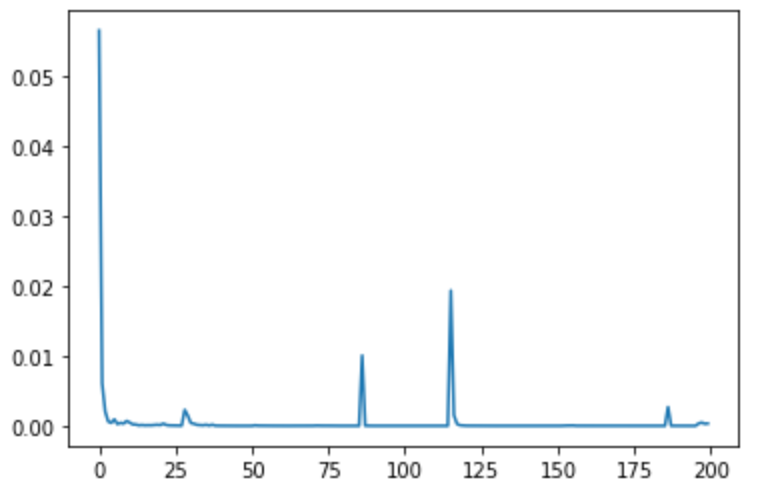
\includegraphics[width=5cm]{fig_dql_loss.jpg}
%& (b)
%&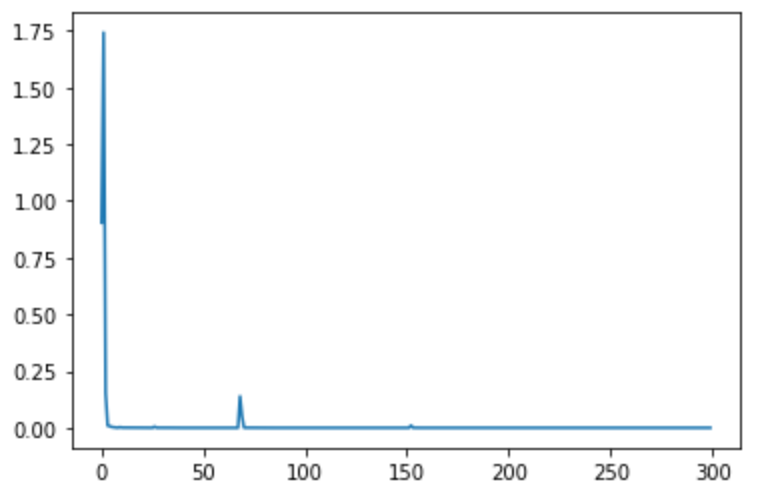
\includegraphics[width=5cm]{fig_dql_loss_long.jpg}
%\end{tabular}
\captionof{figure}{DQL model training loss.}
\label{fig_dql_loss}
\end{center}


\begin{center}
%\begin{tabular}{lclc}
%(a) &
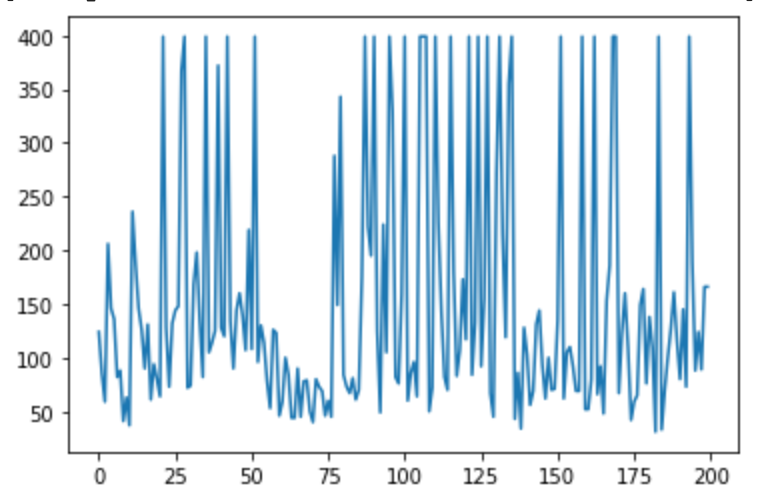
\includegraphics[width=5cm]{fig_dql_steps.jpg}
%& (b)
%&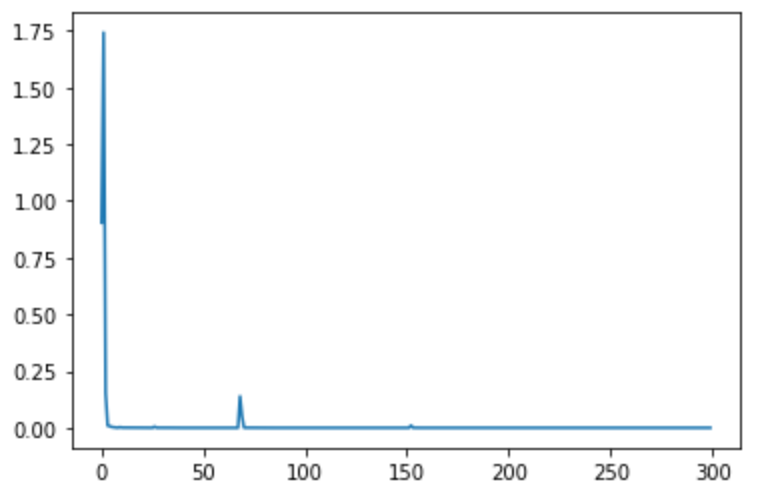
\includegraphics[width=5cm]{fig_dql_loss_long.jpg}
%\end{tabular}
\captionof{figure}{DQL model steps before ``done''.}
\label{fig_dql_steps}
\end{center}
%\section{}\label{question2}

\subsection{}
1st step - no reward.
Thereafter: each step reward of 1 discounted by $\gamma$.
Hence 
\begin{equation*}
V_{a_1}(s_0) = Q(a_1, s_0) = \sum_{t=0}^\infty r_t\gamma^t = 0 + \sum_{t=1}^\infty \gamma^t = \frac{\gamma}{1-\gamma}
\end{equation*}

\subsection{}
1st step - reward of $\frac{\gamma^2}{1-\gamma}$.
Thereafter: each step reward of 0.
Hence 
\begin{equation*}
V_{a_2}(s_0) = Q(a_2, s_0)= \sum_{t=0}^\infty r_t\gamma^t = \frac{\gamma^2}{1-\gamma} \sum_{t=1}^\infty 0\times \gamma^t = \frac{\gamma^2}{1-\gamma} = \gamma Q(a_1, s_0) < Q(a_1, s_0)
\end{equation*}
as $0<\gamma<1$, hence choosing $a_1$ is optimal.

\subsection{}
Bellman value iteration is $V^{(n)}(s_0) = \max_{i\in{1,2}}Q^n (a_i, s_0)$. At iteration $n$, 
\begin{align*}
Q^{(n)}(a_2, s_0) =& \frac{\gamma^2}{1-\gamma} \\
Q^{(n)}(a_1, s_0) =& 0 + \sum_{t=1}^{n-1} \gamma^t = \frac{\gamma (1-\gamma^n) }{1-\gamma} 
\end{align*}
The algorithm will choose $a_1$ for all $k\geq n*$ such that
\begin{align*}
Q^{(n*)}(a_2, s_0) \leq & Q^{(n*)}(a_1, s_0) \\
\frac{\gamma^2}{1-\gamma} \leq & \frac{\gamma (1-\gamma^{n^*}) }{1-\gamma} \\
\gamma \leq&  1-\gamma^{n^*} \\
\frac{\log{(1-\gamma)}}{\log{(\gamma)}} \leq & n^*
\end{align*}
Q.E.D.
%\section{}\label{question3}

Let $\tilde{V}$ be some value function, $V_g$ be the greedy value function and $V^*$ be the optimal value function. Let $\mathbb{S}$ and $\mathbb{A}$ be the state and action spaces, respectively. Let $\epsilon>0$.

For value function $V$ and $s\in \mathbb{S}$ define $L_V(s) = |V(s) - V^*(s)|$ which is the value loss if we choose a sub-optimal policy.

\subparagraph{CLAIM} $|\tilde{V} - V^*|<\epsilon \Rightarrow <\frac{2\epsilon \gamma}{1-\gamma}$.

\subparagraph{PROOF}

Let $\bar{s} = \argmax_{s\in\mathbb{S}} L_{\tilde{V}}(\bar{s})$. This exists by the assumption in CLAIM.

Let $a\mathbb{A}$ be the optimal choice $\pi^*(\bar{s}) = a$ and $b$ be the greedy choice $\pi_g(\bar{s})=b$.

Because $b$ is chosen with greedy policy, it has to be at least as good as $a$:
\begin{equation}
\tilde{V}(s) = R(\bar{s},a)+\gamma \sums{a} \tilde{V} (s') \leq R(\bar{s},b) + \sums{b} \tilde{V}(s')
\label{eq1}
\end{equation}
By assumed property, $ V^*(s) - \epsilon< \tilde{V}(s) <V^*(s) + \epsilon, \forall s\in\mathbb{S}$, hence \eqref{eq1} gives
\begin{equation*}
R(\bar{s},a)+\gamma \gamma \sums{a} \left(V^* (s')-\epsilon\right) \leq R(\bar{s},b) + \gamma \sums{b} \left(V^*(s')+\epsilon \right)
\label{eq2}
\end{equation*}

hence
\begin{equation}
R(\bar{s},a)-R(\bar{s},b) \leq 2\gamma \epsilon + \gamma \sum_{s'\in\mathbb{S}}\left( P(s' | \bar{s},b) V^*(s') - P(s' | \bar{s}, a) V^*(s')\right)
\label{eq3}
\end{equation}

Because $\bar{s}$ was chosen so that it maximizes $L_V(s)$ for an arbitrary value function $V$, in particular it maximizes the loss for the greedy policy value function $L_{V_g}$, hence, using the fact that $g$ is the greedy policy choice, as well as \eqref{eq3} we have
\begin{align*}
L_{V_g}(\bar{s}) = & V^*(\bar{s}) - V_g(\bar{s}) \\
= & R(\bar{s},a)-R(\bar{s},b) + \gamma \sum_{s'\in\mathbb{S}}\left( P(s' | \bar{s},a) V^*(s') - P(s' | \bar{s}, b) V_g^*(s')\right) \\
\leq & 2\epsilon \gamma + \gamma \sum_{s'\in\mathbb{S}}\left( P(s' | \bar{s},b) V^*(s') - P(s' | \bar{s},a) V^*(s') + P(s' | \bar{s}, a) V^*(s') - P(s' | \bar{s},b) V_g^*(s')\right)\\
&= 2\epsilon \gamma + \gamma \sum_{s'\in\mathbb{S}}\left( P(s' | \bar{s},b) V^*(s') - P(s' | \bar{s},b) V_g(s')\right)\\
&=2\epsilon \gamma + \gamma \sums{b} L_{V_g}(s')\\
&\leq 2\epsilon\gamma + \gamma \sums{b} L_{V_g}(\bar{s})
\end{align*}
rearranging we get that for every $s\in\mathbb{S}$
\begin{equation*}
L_{V_g}(s) = \leq L_{V_g}(\bar{s}) \leq \frac{2\epsilon\gamma}{1-\gamma}
%\label{eq2}
\end{equation*}
Q.E.D.


%\input{AccuracyLoss}

\end{document}